\chapter{Bioinformatics}

In this chapter I present an overview of some interesting and important bioinformatical problems, particularly protein folding, which is one of the central problems related to drug discovery\cite{BockenhauerAlgoBioinfo}.

\section{Computational problems in bioinformatics}

\subsection{DNA sequencing and the Human Genome Project}

The complete genetic material of a human being is called the human genome, which is contained in the nucleus of every single cell of the human body and is replicated during cell division. The human genome consists of 46 chromosomes in total, each of which contains a single deoxyribonucleic acid, or DNA molecule for short. A DNA molecule is two twisting, paired strands (called the double helix structure) and is made up of around 3.2 billion pairs of nucleotide bases. Nucleotides are usually denoted by the letters A,T,C and G, with A-T and C-G forming pairs together. A sequence of nucleotides, that together encode the synthesis of a specific protein or RNA is called a gene.

\begin{figure}[H]
    \centering
    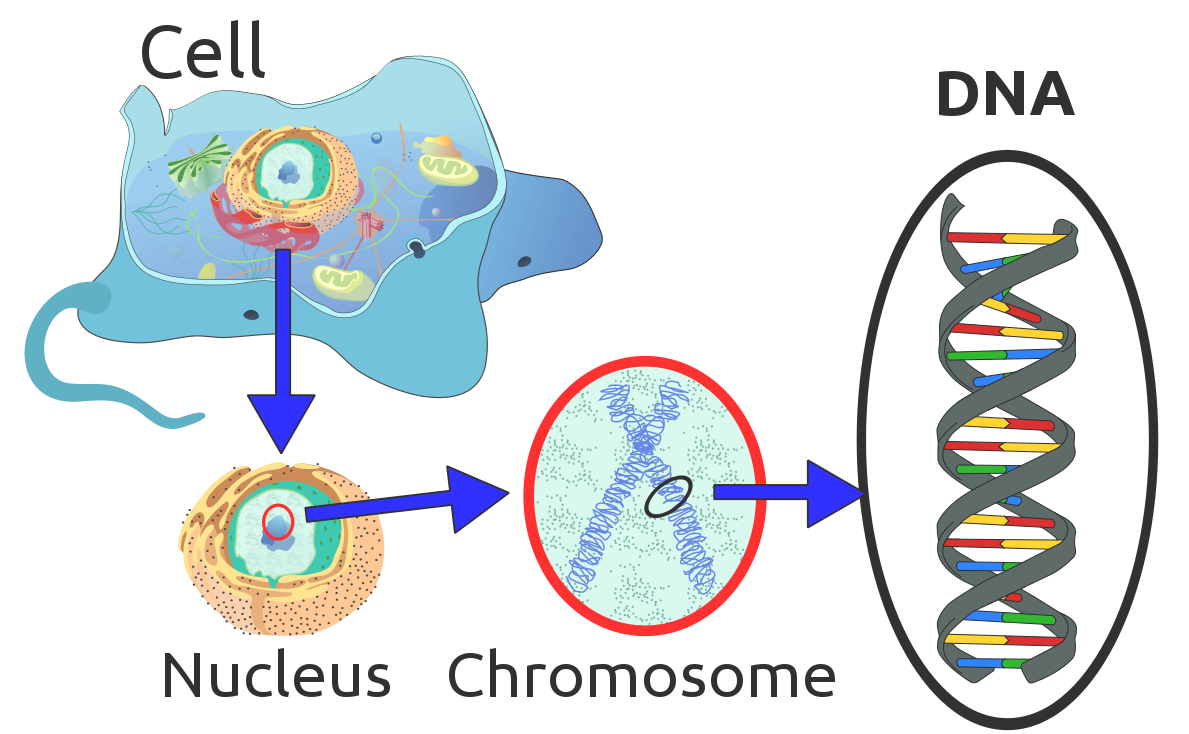
\includegraphics[width=0.8\textwidth]{figures/bioinformatics/dna.png}
    \caption{DNA structure, \href{https://commons.wikimedia.org/wiki/File:Eukaryote\_DNA-en.svg}{(Source: Wikimedia Commons)}}
\end{figure}

Research into the human genome has started with the discovery of the double helix structure of the DNA molecule in 1953, by Francis Crick and James Watson. The Human Genome Project\cite{CollinsHumanGenome1995} was launched in 1990, an international research effort to identify the function of all 50,000 to 100,000 genes of the complete human genetic material and was completed in early 2022\cite{zahn_filling_2022}. Apart from injuries, nearly all human medical conditions are related to mutations at specific locations in the structure and function of the genetic material\cite{CollinsHumanGenome1995}, so identifying changes in an individual's DNA sequence can be an indispensable tool for predicting and preventing disease, while providing individualized care. This requires a quick method of sequencing specific parts of a person's DNA and comparing them to a healthy variant.

From a computer science viewpoint, a simplified model of the DNA is a string, consisting of the 4 letters (A,C,T and G) from one of the strands of the physical molecule. (However, this model omits the 3D spatial structure.) Due to the limits of our technology, current methods enable us to read up to 1000 consecutive letters from a single sample. To sequence a longer string, we can break the molecule into sufficiently smaller fragments and sequence them individually. Unfortunately, in this process the order in which the fragments originally occured is lost. One possible approach to deal with this problem is to create copies of the DNA molecule we are interested in and randomly break each of these copies into fragments. With high probability, the resulting fragments from different copies will overlap with each other. Then, the task becomes reconstructing the original string from these fragments, while taking into account the possible errors in our biological measurements. The possible number of fragment orderings is enormously large, hence why a brute force algorithm does not suffice for solving this task.\cite{CollinsHumanGenome1995}

Between any two humans, the amount of genetic variation is estimated to be around 0.6\%\cite{the_1000_genomes_project_consortium_global_2015}. This enables us to use the targeted part of the genome sequence preassembled by the Human Genome Project and align our obtained DNA sequence fragments to the best fitting position in it to obtain the full string of our DNA. Algorithms such as the Smith–Waterman algorithm and the Needleman–Wunsch algorithm can perform this sequence alignment task efficiently.

\subsection{Protein folding}

Proteins are one of the fundamental building blocks of the human body. They play an essential role in our immune system response, transportation of molecules throughout the body, the catalysation of metabolic reactions and signal transmission. Protein molecules consist of a single, long chain of amino acids. While several amino acid molecules exist in nature, only 20 of those are present in proteins.\cite{BockenhauerAlgoBioinfo}

The 20 standard amino acids can be seen in Table \ref{aminoacids20}. The most important property of these is their affinity to water: Some amino acids are polar (hydrophilic), commonly denoted by a P, which means they can establish hydrogen bonds with $H_2O$ molecules. In contrast, others are hydrophobic (nonpolar), commonly denoted by an H, which do not establish these bonds with water.

\begin{table}[H]
\centering
\begin{tabular}{|l|ccc|}
\hline
Name          & Abbreviation & Code & Polarity \\
\hline
Alanine       & Ala & A & H \\
Valine        & Val & V & H \\
Leucine       & Leu & L & H \\
Isoleucine    & Ile & I & H \\
Phenylalanine & Phe & F & H \\
Proline       & Pro & P & H \\
Methionine    & Met & M & H \\
Tryptophan    & Trp & W & H \\
\hline
Arginine      & Arg & R & P \\
Asparagine    & Asn & N & P \\
Aspartic acid & Asp & D & P \\
Cysteine      & Cys & C & P \\
Glutamic acid & Glu & E & P \\
Glutamine     & Gln & Q & P \\
Glycine       & Gly & G & P \\
Histidine     & His & H & P \\
Lysine        & Lys & K & P \\
Serine        & Ser & S & P \\
Threonine     & Thr & T & P \\
Tyrosine      & Tyr & Y & P \\
\hline
\end{tabular}
\caption{Aminoacids in proteins}
\label{aminoacids20}
\end{table}

The functionality and role of a protein are determined by its spatial structure, of which four levels are distinguished.

\textbf{Primary structure}: The sequence of amino acids in the protein.

\begin{figure}[H]
    \centering
    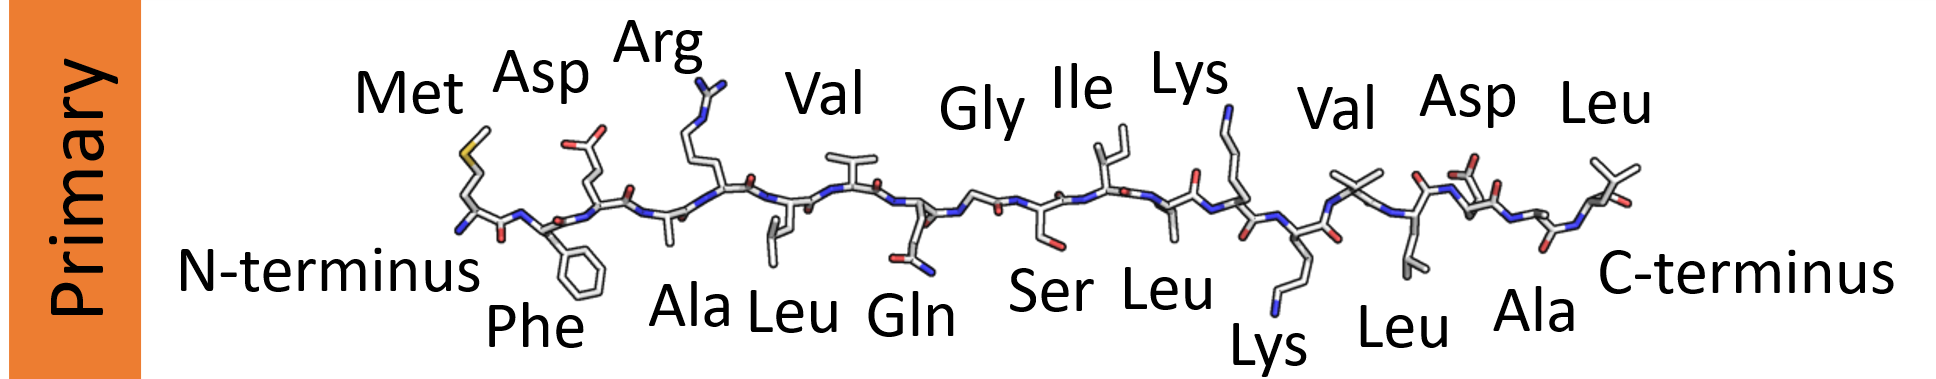
\includegraphics[width=\textwidth]{figures/bioinformatics/protein_structure_primary.png}
    \caption{Primary structure of the protein PCNA\\(Author: Thomas Shafee, \href{https://en.wikipedia.org/wiki/File:Protein\_structure\_(full).png}{Source})}
\end{figure}

\textbf{Secondary structure}: Created by the interactions between the atoms along the chain of amino acids, forming substructures ($\alpha$-helices, $\beta$-sheets, loops).

\begin{figure}[H]
    \centering
    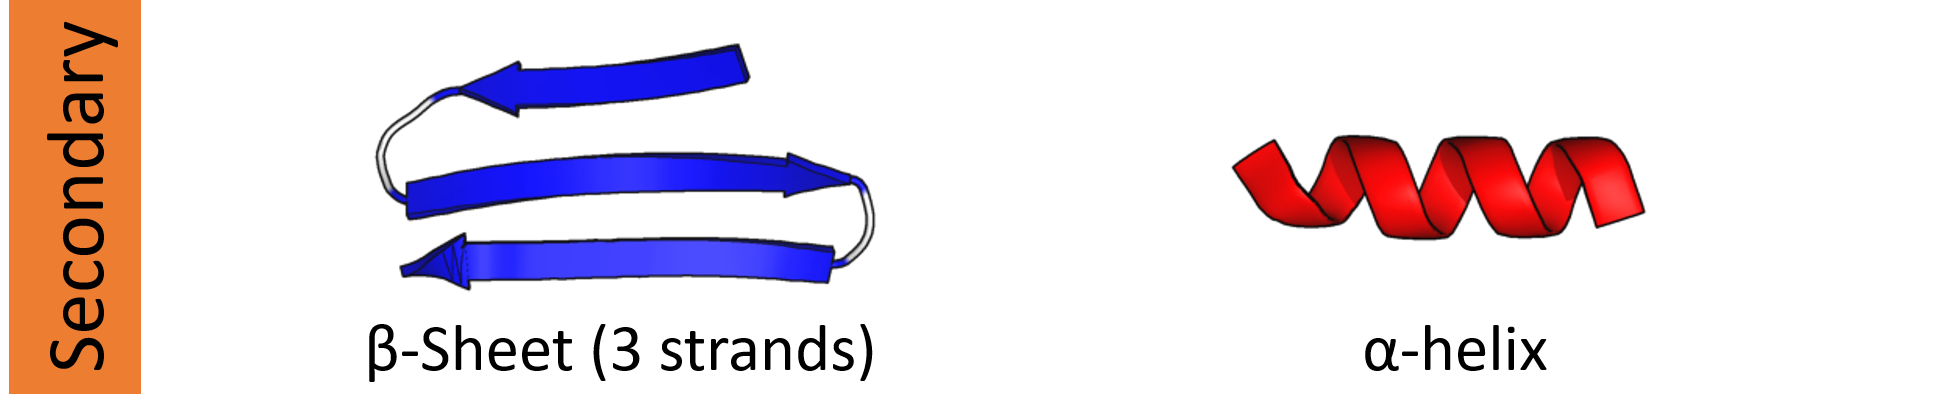
\includegraphics[width=\textwidth]{figures/bioinformatics/protein_structure_secondary.png}
    \caption{Secondary structure of the protein PCNA\\(Author: Thomas Shafee, \href{https://en.wikipedia.org/wiki/File:Protein\_structure\_(full).png}{Source})}
\end{figure}

\textbf{Tertiary structure}: The spatial arrangement of all atoms within the chain. Secondary structure elements are grouped together as motifs, and functional units called domains.

\begin{figure}[H]
    \centering
    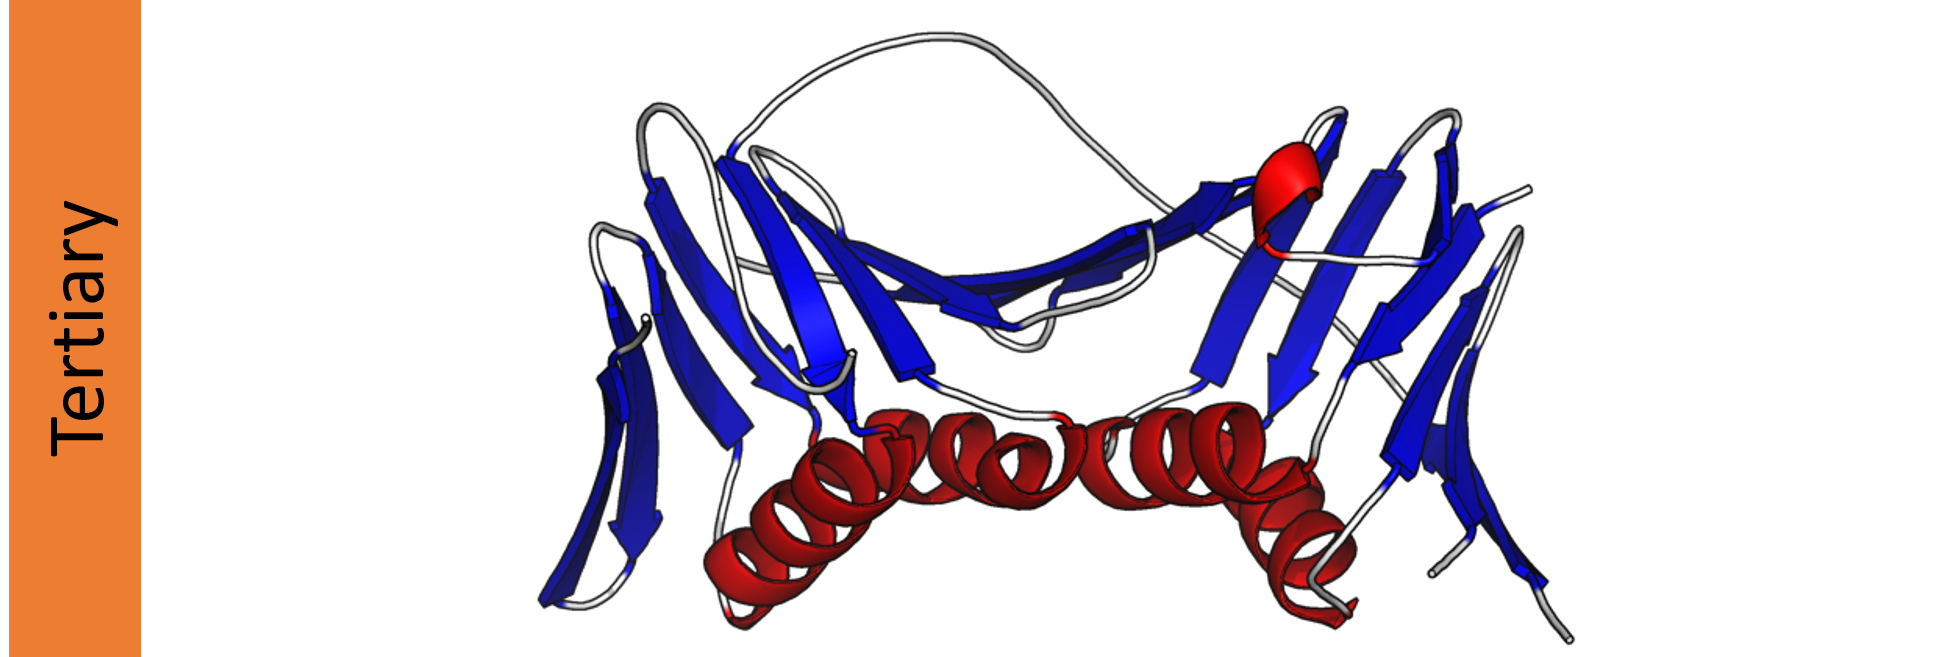
\includegraphics[width=\textwidth]{figures/bioinformatics/protein_structure_tertiary.png}
    \caption{Tertiary structure of the protein PCNA\\(Author: Thomas Shafee, \href{https://en.wikipedia.org/wiki/File:Protein\_structure\_(full).png}{Source})}
\end{figure}

\textbf{Quaternary structure}: Describes the composition of the whole protein from polypeptide subunits and potentially other molecular parts.

\begin{figure}[H]
    \centering
    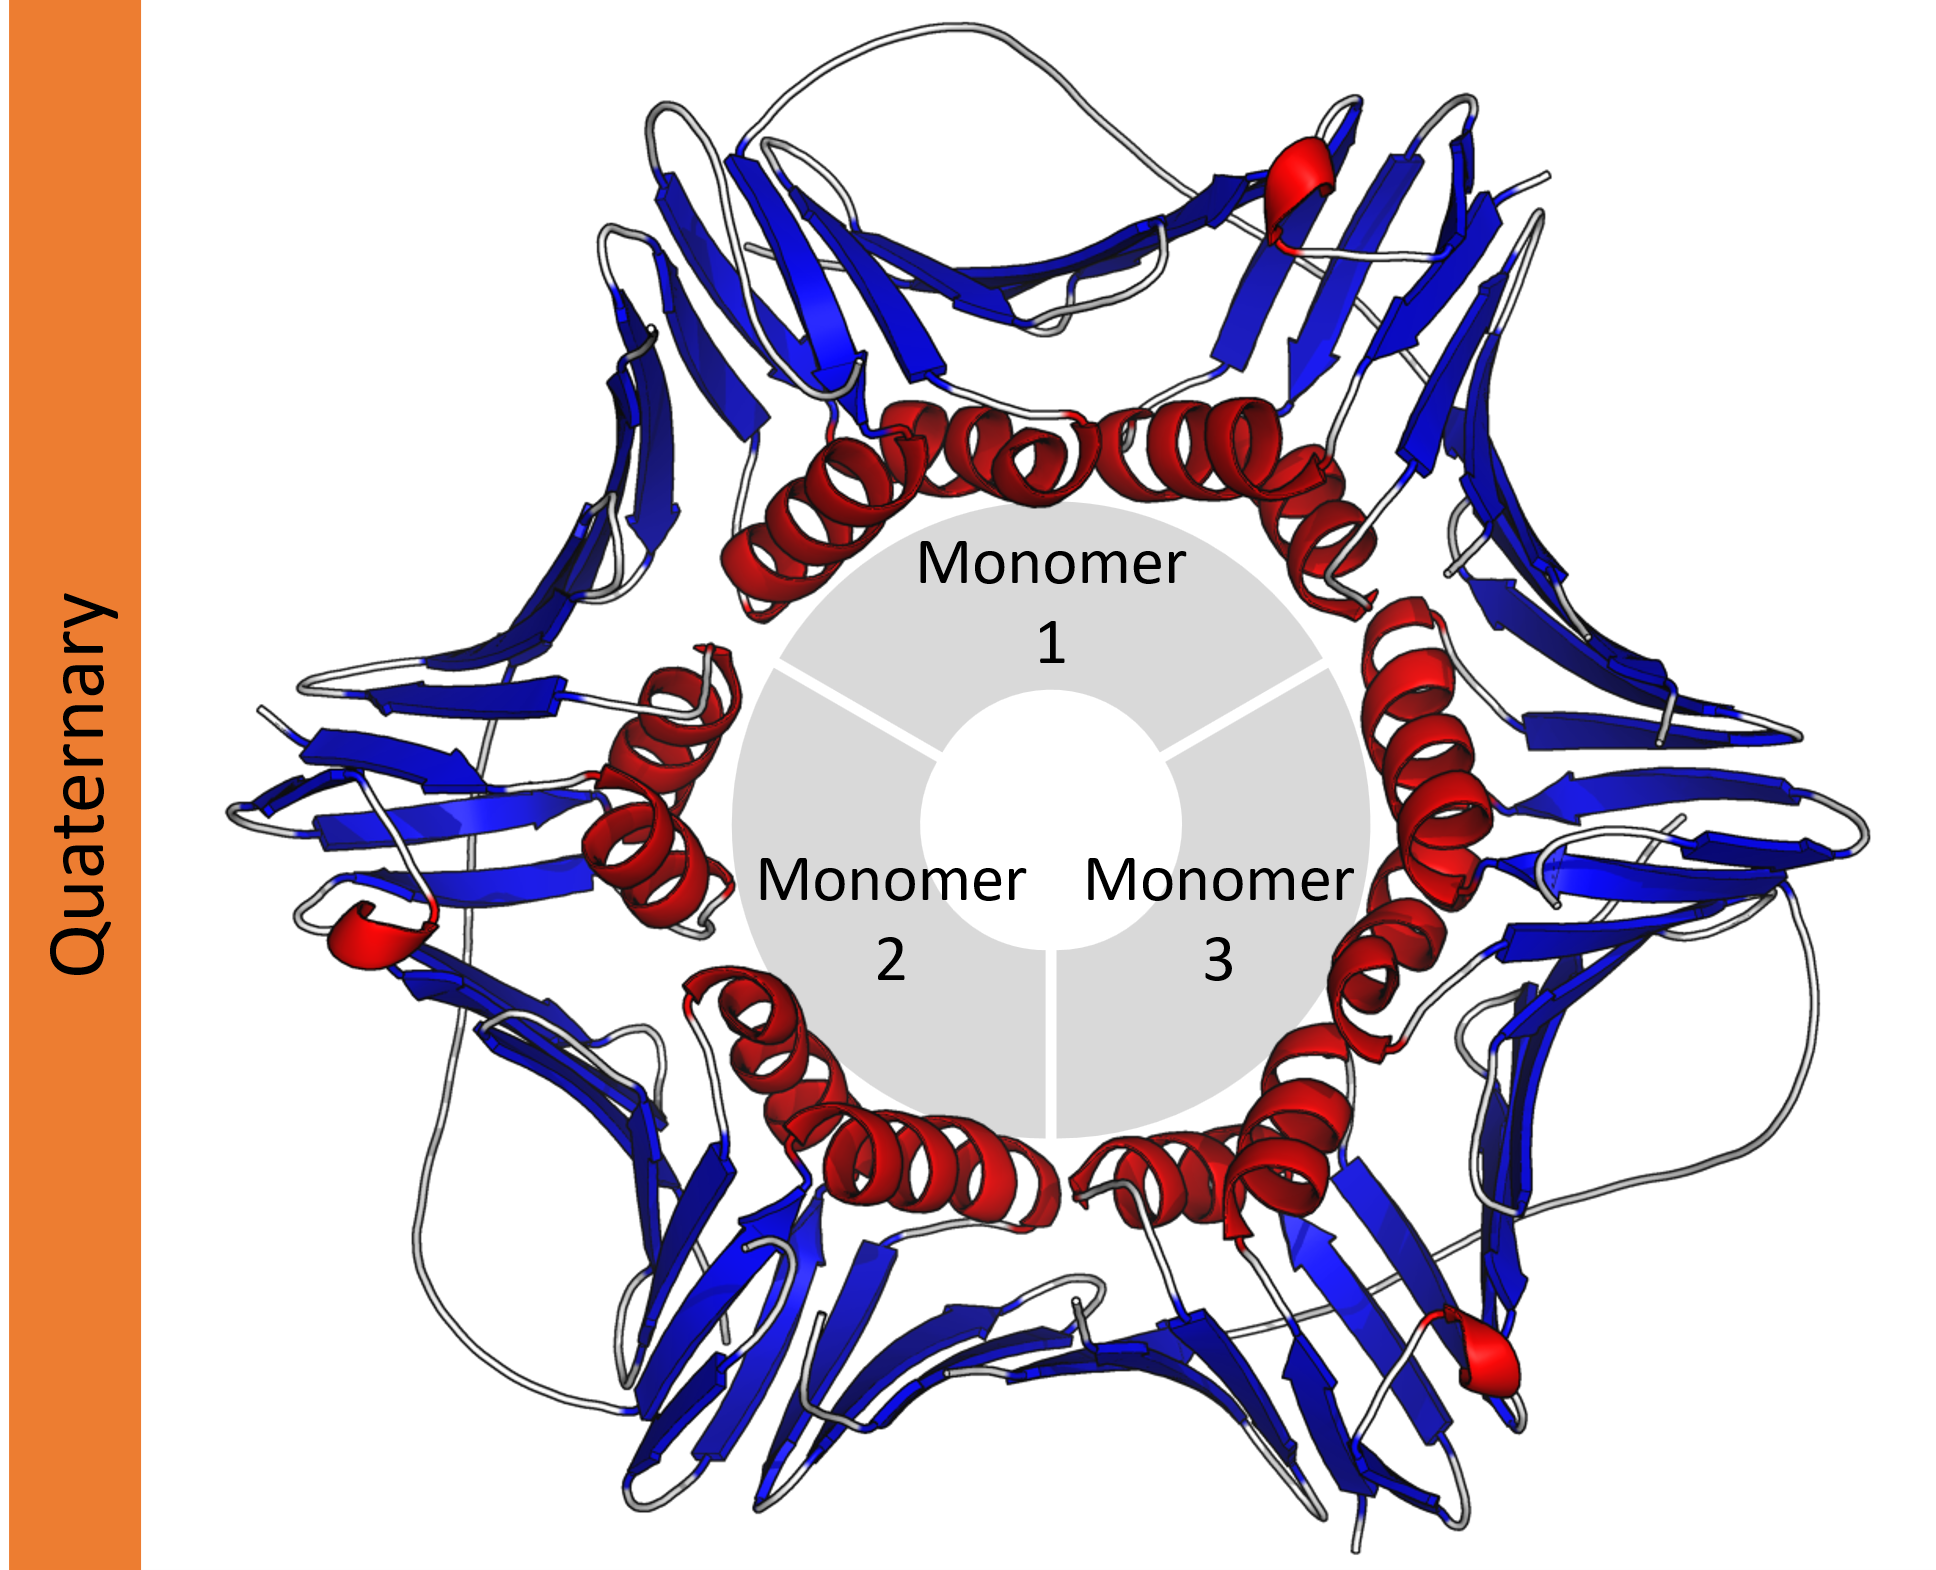
\includegraphics[width=\textwidth]{figures/bioinformatics/protein_structure_quaternary.png}
    \caption{Quaternary structure of the protein PCNA\\(Author: Thomas Shafee, \href{https://en.wikipedia.org/wiki/File:Protein\_structure\_(full).png}{Source})}
\end{figure}

For example, hemoglobin is a protein found in red blood cells whose function is to carry oxygen molecules throughout the blood vessels. The oxygen molecule binds to the hemo groups found in the protein.

\begin{figure}[H]
    \centering
    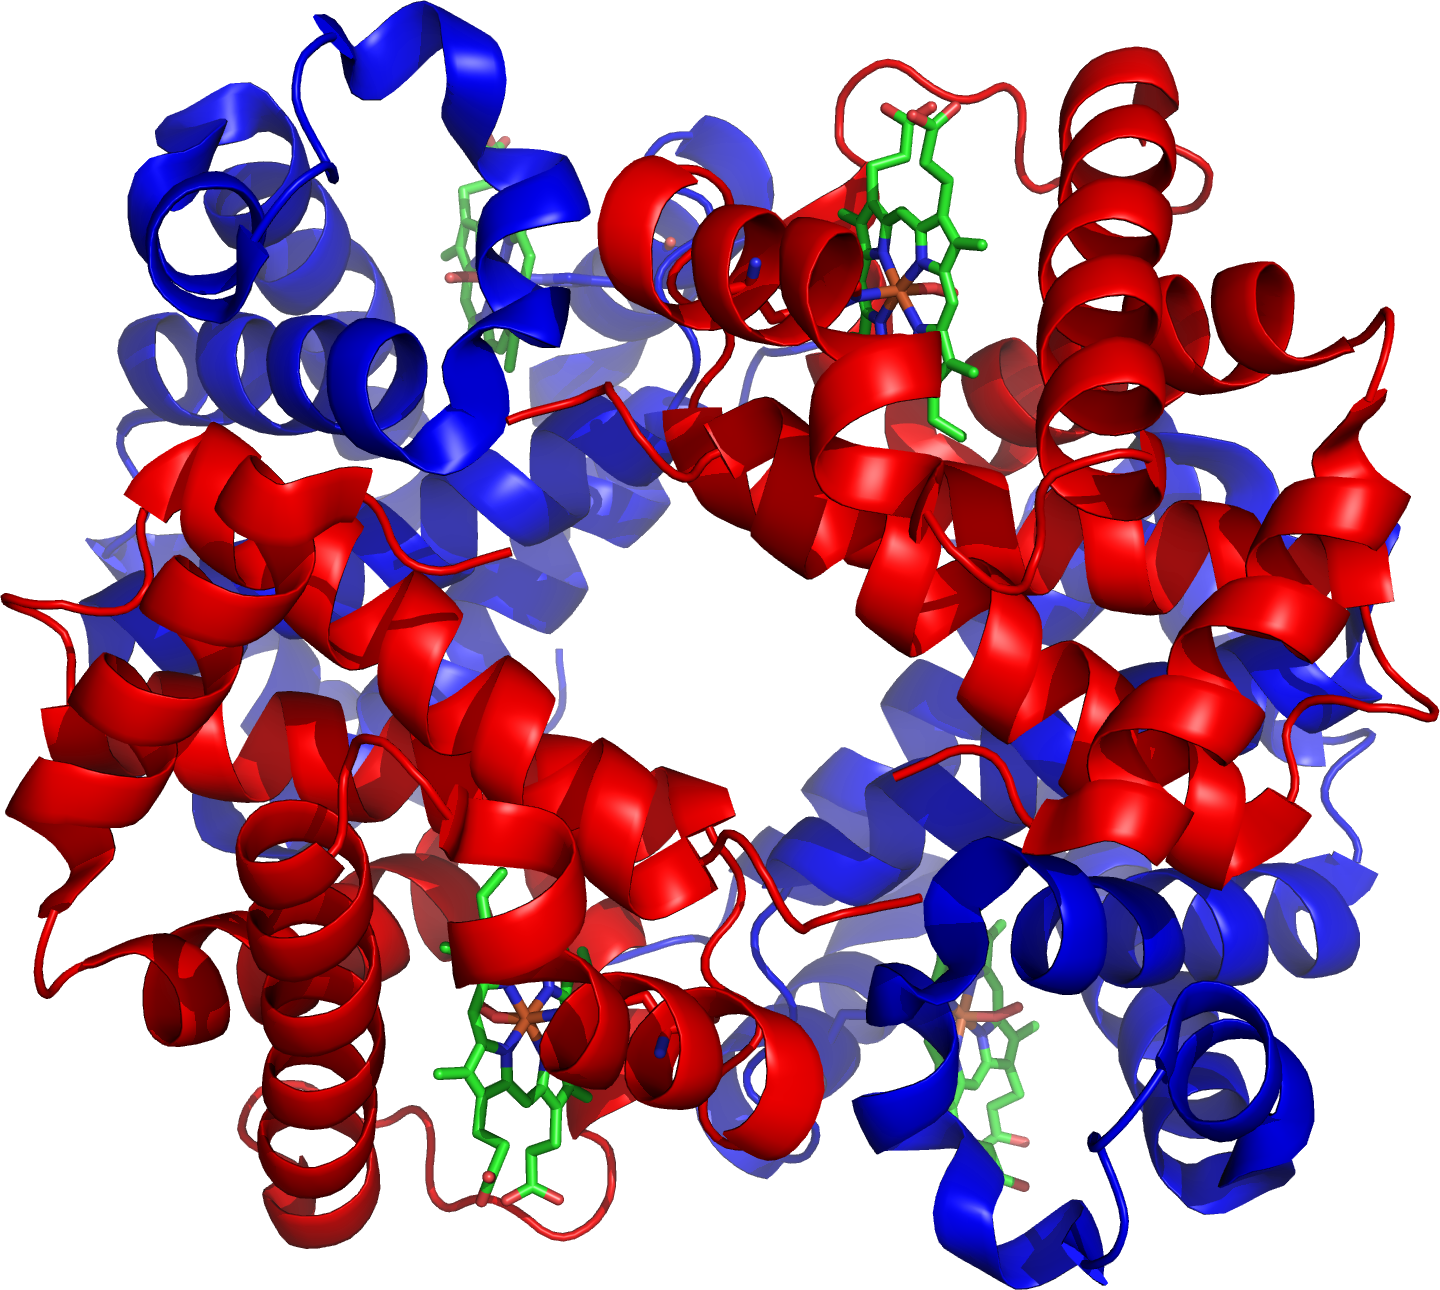
\includegraphics[width=0.7\textwidth]{figures/bioinformatics/hemoglobin.png}
    \caption{Hemoglobin, the iron-containing heme groups are shown in green \\(Author: Richard Wheeler, \href{https://en.wikipedia.org/wiki/File:1GZX\_Haemoglobin.png}{Source})}
\end{figure}

To understand the function of a protein, we must determine its complete 3D structure. While techniques exist to measure a molecule's structure in real life, these are incredibly time-consuming and expensive to perform, even for a single molecule. Consequently, we would like to design algorithms that can predict the complete 3D structure of a protein based on its primary structure or its amino acid sequence. These algorithms are called protein folding algorithms.

\subsubsection{Molecular docking}

Proteins are the primary agents of biological function, as they control the various chemical mechanisms that occur inside the cells. Proteins that act as biological catalysts are called enzymes. Catalysts facilitate various chemical reactions without being consumed in the process. These molecules have a binding site (a 'hole' on their 3D surface), into which only a specific other molecule fits, which is called a substrate. During the chemical reaction, the substrate is turned into other products.  \cite{fionda_networks_2019}

Many human diseases result from abnormal interactions between proteins. In order to prevent disease, we can stop (inhibit) these interactions from happening. This is done by blocking the binding site of the faulty enzyme with another molecule. Conventional medicine uses giant molecules (antibodies) or tiny molecules (like aspirin) to achieve this. The next generation of protein therapeutics currently under development aims to find inhibitors within the family of smaller-sized proteins.
 \cite{ryan_proteinprotein_2005}

In order to inhibit an enzyme's reaction from happening, we must find a protein that folds into a shape that fits into the enzyme's binding site to prevent it from catalyzing a reaction. The analogy of 'lock-and-key' was coined for this by Emil Fischer in 1894. He suggested that the 'lock' describes the enzyme's binding site, and the 'key' describes the missing molecule inhibitor, which has to fit into the 'lock'. \cite{a_molecular_2018} \cite{walker_molecular_2008} The computational task of predicting whether a protein with a known 3D structure will fit inside the binding site of a specific enzyme is called molecular docking.

\begin{figure}[H]
    \centering
    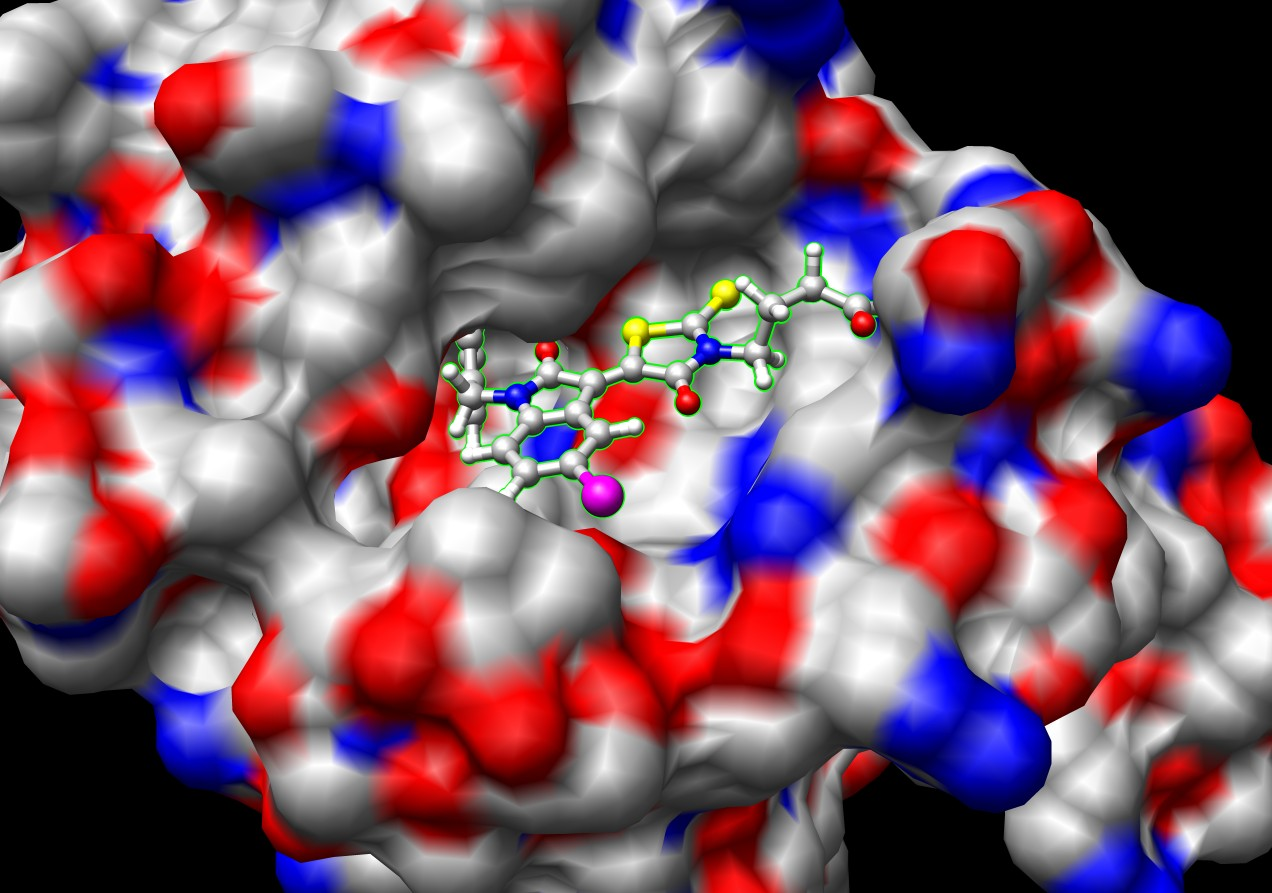
\includegraphics[width=0.7\textwidth]{figures/bioinformatics/molecular_docking.jpg}
    \caption{Molecular docking \\(\href{https://commons.wikimedia.org/wiki/File:Docking.jpg}{Source: Wikimedia Commons})}
\end{figure}

In the molecular docking problem, both the binding site's 3D structure and the protein's 3D structure are represented by a graph. The graph's vertices are the atoms on the surface. The edges represent a chemical bond between the corresponding atoms. The weight of a given edge represents the physical distance between the atoms. Omitting the edge weights, the problem is analogous to subgraph isomorphy (an NP-complete problem), the binding site's graph representation being a subgraph of the inhibitor molecule's entire surface in a graph representation. With the edge weights present, we employ a measure that assigns a score to an isomorphy mapping of the vertices between the two graphs. Typically root mean square deviation (RMSD) is used, which can be defined for two sets of (ordered) points. The mapping achieving the highest score is the best theoretical fit for the molecule.
 \cite{wang_protein_2021}
 
\subsubsection{The HP modell by Dill}

In the molecular docking task, the candidate protein has already been selected with its 3D structure known. For the purpose of drug discovery, we are searching for the best possible protein as well, which is why databases of proteins with their predicted 3D structures are being worked on, such as \href{https://www.uniprot.org/}{https://www.uniprot.org/}, or \href{https://alphafold.ebi.ac.uk/}{https://alphafold.ebi.ac.uk/}. \cite{senior_improved_2020}

Modelling and predicting the complete four levels of protein structure is a complex task. Interestingly, simplified models exist that can be experimentally shown to achieve a reasonable approximation. One of these models was given by Dill et al. in 1995. (republished in 2008).\cite{dill_principles_2008} 

The HP model replaces all protein's amino acids by their water affinity categories: polar (P) and hydrophobic (H), or 0 and 1. Then, the protein can be represented by a sequence consisting of letters H and P of the length equal to its amino acid number. Then, this chain is embedded in either a two- or a three-dimensional grid. The letters must be placed in the grid's intersections so that consecutive letters are in adjoining intersections (either to the up, down, left or right directions and above or under in the 3D case) while the chain is not allowed to cross itself over. Then a scoring of the placement is determined by the count of the all pairs of non-covalently bonded (non-consecutive) but neighbouring H letters on the grid. This captures the idea of energy minimization, in which the hydrophobic molecules tend to be close to each other and thus avoid exposure, while the polar molecules are neutral, since in the cell, all molecules are immersed in ''water'', the energy is best conserved by forming an external shell from their water-liking parts and hiding their water-disliking parts in the inside.

\begin{figure}[H]
    \centering
    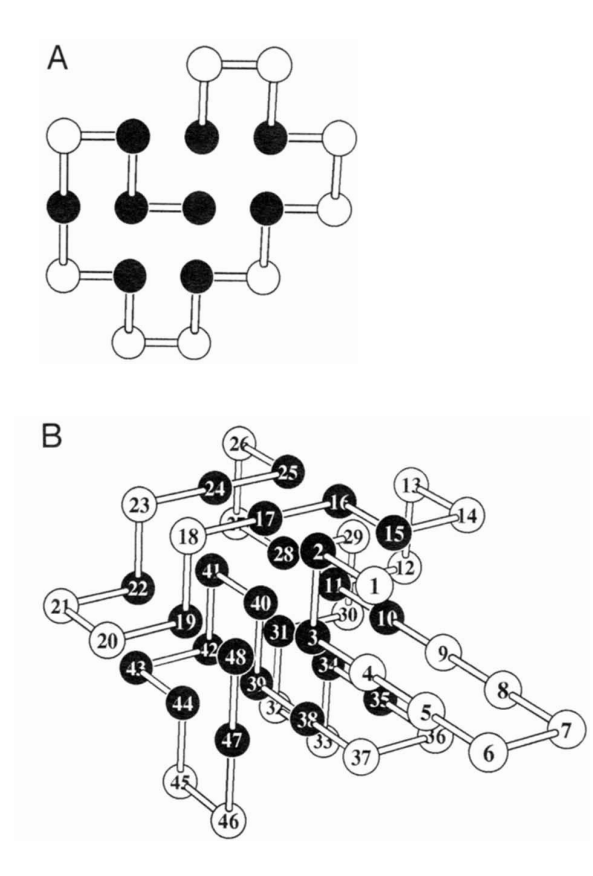
\includegraphics[width=0.6\textwidth]{figures/bioinformatics/hp_model.png}
    \caption{Examples of a HP chain embedded in 2D and 3D space\\(H represented in black, P in white)\cite{dill_principles_2008}}
\end{figure}

Even this simplified problem is proven to be NP-hard, sinc a reduction from the Hamiltonian-cycle problem can be shown \cite{crescenzi_complexity_1998}. We could achieve a slightly more complex model, by keeping the grid but reverting back to 20 possible letters, corresponding to the 20 possible amino-acids and employing a scoring matrix for all possible pairs of neighbours, however the two-dimensional HP model has been found to be the best match of the experimental results among all of these approximations. \cite{crescenzi_complexity_1998}

